\newpage
\section{Ogólne określenie wymagań}		%1
%Określenie celu pracy, co chcemy uzyskać, jakie przewidujemy wyniki

\hspace{0.60cm}
Niniejszy rozdział przedstawia szczegółowe opisy wymagań technicznych, funkcjonalnych. Głównym zadaniem jest stworzenie w pełni funkcjonalnej aplikacji w języku C++ operującej na strukturze danych drzewa poszukiwań binarnych (ang. \textit{Binary Search Tree} -- BST) z wykorzystaniem kontenerów biblioteki standardowej STL, a także przeprowadzenie pełnego cyklu integracji i kontroli wersji za pomocą platformy GitHub w zespole dwuosobowym.

\subsection{Wprowadzenie teoretyczne i cel projektu}

\hspace{0.60cm}
Drzewo poszukiwań binarnych jest dynamiczną strukturą danych, w której każdy węzeł zawiera klucz (w naszym przypadku wartość liczbową) oraz co najwyżej dwóch potomków, nazywanych tradycyjnie lewym i prawym dzieckiem. Kluczową własnością drzewa BST jest porządek, w którym dla każdego węzła $N$:
\begin{itemize}
    \item Wszystkie klucze znajdujące się w lewym poddrzewie węzła $N$ mają wartości ściśle mniejsze od wartości klucza węzła $N$.
    \item Wszystkie klucze znajdujące się w prawym poddrzewie węzła $N$ mają wartości większe lub równe wartości klucza węzła $N$.
\end{itemize}

\hspace{0.60cm}
Właściwość ta pozwala na wysoce wydajne wyszukiwanie elementów, osiągające złożoność obliczeniową $O(\log_2 n)$ w przypadku drzew zrównoważonych. W najgorszym przypadku (gdy wprowadzane dane są już posortowane, a drzewo ulega zdegenerowaniu do postaci listy jednokierunkowej) złożoność ta wzrasta do $O(n)$. Cel projektu obejmuje nie tylko implementację samego drzewa, ale również opracowanie stabilnego modułu serializacji danych (zapis/odczyt binarny oraz tekstowy) oraz stworzenie przejrzystego interfejsu konsolowego z obsługą menu.

\subsection{Szczegółowe wymagania funkcjonalne}

\hspace{0.60cm}
Wymagania postawione przed aplikacją podzielono na grupy funkcjonalne, które zostały wyszczególnione w poniższym zestawieniu:

\begin{enumerate}
    \item \textbf{Zarządzanie strukturą drzewa BST:}
    \begin{itemize}
        \item Dynamiczne dodawanie nowego elementu (węzła) do istniejącego lub pustego drzewa z zachowaniem własności BST.
        \item Usuwanie wskazanego elementu z drzewa z poprawną reorganizacją wskaźników (przypadki: węzeł bez dzieci, z jednym dzieckiem, z dwójką dzieci).
        \item Całkowite czyszczenie drzewa (zwolnienie pamięci wszystkich węzłów, np. przy użyciu przejścia \textit{postorder}).
        \item Wyszukiwanie ścieżki od korzenia do wybranego elementu i prezentacja kolejnych węzłów na tej ścieżce.
    \end{itemize}

    \item \textbf{Wizualizacja i reprezentacja danych:}
    \begin{itemize}
        \item Wyświetlanie graficzne lub strukturalne drzewa w konsoli.
        \item Wybór metody przechodzenia przez użytkownika podczas wyświetlania: \textit{preorder} (root-left-right), \textit{inorder} (left-root-right) oraz \textit{postorder} (left-right-root).
    \end{itemize}

    \item \textbf{Obsługa plików i wejścia/wyjścia (I/O):}
    \begin{itemize}
        \item Zapis wygenerowanego drzewa do czytelnego pliku tekstowego (\texttt{.txt}).
        \item Dedykowana klasa narzędziowa do binarnego zapisu i odczytu drzewa (\texttt{.bin}).
        \item Wczytywanie pliku tekstowego z cyframi/liczbami w celu zbudowania nowego drzewa lub dołączenia danych do drzewa istniejącego.
    \end{itemize}

    \item \textbf{Interfejs i architektura programu:}
    \begin{itemize}
        \item Funkcja \texttt{main} serwująca interaktywne menu tekstowe z pętlą obsługi zdarzeń i bezpiecznym wyjściem z programu.
        \item Pełny podział modularny: każda klasa zdeklarowana w odrębnym pliku nagłówkowym (\texttt{.h}) i zaimplementowana w pliku źródłowym (\texttt{.cpp}).
    \end{itemize}
\end{enumerate}

\subsection{Architektura modularna i struktura klas}

\hspace{0.60cm}
Zgodnie z zasadami programowania obiektowego (OOP) aplikacja została podzielona na trzy główne komponenty. Taki podział gwarantuje wysoką spójność wewnętrzną (ang. \textit{cohesion}) oraz niskie sprzężenie (ang. \textit{coupling}).

\hspace{0.60cm}
Wykaz poszczególnych modułów programu przedstawiono w tabeli \ref{tab:struktura_klas} (s. \pageref{tab:struktura_klas}).

\begin{tabela}
	{Struktura klas i modułów aplikacji}
	{Struktura klas i modułów aplikacji}
	{
		\begin{tabular}{|l|l|p{6.5cm}|} \hline
			\textbf{Nazwa pliku} & \textbf{Moduł / Klasa} & \textbf{Odpowiedzialność w systemie} \\ \hline
			\texttt{BST.h / .cpp} & \texttt{BSTTree} & Klasa główna drzewa: wstawianie, usuwanie, przechodzenie, wyszukiwanie ścieżki. \\ \hline
			\texttt{FileManager.h / .cpp} & \texttt{FileHandler} & Zapis/odczyt binarny reprezentacji drzewa, wczytywanie liczb z pliku tekstowego. \\ \hline
			\texttt{Node.h } & Node (struktura) & Przechowuje dane oraz położenie elementu \\ \hline
			\texttt{main.cpp} & Interfejs (CLI) & Główna pętla programu, sterowanie menu, przyjmowanie danych od użytkownika. \\ \hline
		\end{tabular}
	}
	\label{tab:struktura_klas}
\end{tabela}

\hspace{0.60cm}
Listing \ref{lst:listing-cpp} (s. \pageref{lst:listing-cpp}) prezentuje przykładowy interfejs klasy \texttt{BSTTree} zawierający deklaracje kluczowych metod operujących na drzewie.

\begin{lstlisting}[caption=Deklaracja nagłówkowa klasy BSTTree, label={lst:listing-cpp}, language=C++]
#ifndef BST_H
#define BST_H

#include <iostream>
#include <vector>
#include <string>

struct Node {
    int value;
    Node* left;
    Node* right;
    Node(int val) : value(val), left(nullptr), right(nullptr) {}
};

class BSTTree {
private:
    Node* root;
    void clearRecursive(Node* node);
    void preorderRecursive(Node* node) const;
    void inorderRecursive(Node* node) const;
    void postorderRecursive(Node* node) const;
    bool findPathRecursive(Node* node, int target, std::vector<int>& path) const;

public:
    BSTTree();
    ~BSTTree();
    
    void insert(int value);
    bool remove(int value);
    void clear();
    std::vector<int> getPath(int target) const;
    
    void displayPreorder() const;
    void displayInorder() const;
    void displayPostorder() const;
    
    Node* getRoot() const { return root; }
};

#endif // BST_H
\end{lstlisting}

\subsection{Algorytmy przechodzenia oraz operacji na plikach}

\hspace{0.60cm}
Kluczowym elementem projektu jest implementacja trzech podstawowych algorytmów przejścia przez strukturę drzewiastą. Każda z tych metod realizuje specyficzny porządek przetwarzania danych:

\begin{itemize}
    \item \textbf{Preorder (współrzędny):} Przetwarzany jest najpierw węzeł bieżący, następnie jego lewe poddrzewo, a na końcu prawe poddrzewo. Przejście to jest wykorzystywane m.in. do tworzenia kopii drzewa lub do zapisu w pliku w sposób umożliwiający odtworzenie identycznej struktury.
    \item \textbf{Inorder (poprzeczny):} Najpierw przetwarzane jest lewe poddrzewo, potem węzeł bieżący, a na końcu prawe poddrzewo. Dla drzewa BST przejście to gwarantuje wypisanie wszystkich zgromadzonych wartości w kolejności rosnącej.
    \item \textbf{Postorder (odwrotny):} Najpierw przetwarzane są lewe i prawe poddrzewo, a dopiero na końcu węzeł bieżący. Jest to idealne rozwiązanie przy zwalnianiu pamięci (usuwaniu drzewa), gdyż dzieci są niszczone przed swoim rodzicem.
\end{itemize}

\hspace{0.60cm}
W drugiej klasie (\texttt{FileHandler}) zaimplementowano funkcjonalność operowania na plikach w dwóch standardach. Tabela \ref{tab:tablica001} (s. \pageref{tab:tablica001}) zawiera opis zastosowania poszczególnych formatów zapisu.

\begin{tabela}
	{Porównanie formatów plików wykorzystywanych w projekcie}
	{Porównanie formatów plików wykorzystywanych w projekcie}
	{
		\begin{tabular}{|p{3.5cm}|p{4.5cm}|p{4.5cm}|} \hline
			\textbf{Cecha} & \textbf{Plik Tekstowy (.txt)} & \textbf{Plik Binarny (.bin)} \\ \hline
			\textbf{Forma danych} & Znaki ASCII (cyfry oddzielone spacją/nową linią) & Bajtowa reprezentacja struktur w pamięci \\ \hline
			\textbf{Zastosowanie} & Wczytywanie danych wejściowych, eksport widoku & Szybka serializacja i deserializacja stanu drzewa \\ \hline
			\textbf{Odczytywalność} & Bezpośrednio widoczna w edytorze tekstu & Wymaga dedykowanego parsera / programu \\ \hline
		\end{tabular}
	}
	\label{tab:tablica001}
\end{tabela}

\hspace{0.60cm}
Listing \ref{lst:listing-cpp2} (s. \pageref{lst:listing-cpp2}) przedstawia fragment kodu odpowiedzialny za binarny zapis struktury drzewa do pliku.

\begin{lstlisting}[caption=Zapis binarny węzłów drzewa BST do pliku, label={lst:listing-cpp2}, language=C++]
#include "FileHandler.h"
#include <fstream>

bool FileHandler::saveBinary(const std::string& filename, const BSTTree& tree) {
    std::ofstream outFile(filename, std::ios::binary);
    if (!outFile.is_open()) {
        return false;
    }
    
    // Zapytanie o strukture i zapis pre-order do pliku binarnego
    std::vector<int> data;
    // ... zbieranie danych do wektora ...
    
    size_t count = data.size();
    outFile.write(reinterpret_cast<const char*>(&count), sizeof(count));
    for (int val : data) {
        outFile.write(reinterpret_cast<const char*>(&val), sizeof(val));
    }
    
    outFile.close();
    return true;
}
\end{lstlisting}

\subsection{Wymagania dotyczące pracy w zespole i systemu Git}

\hspace{0.60cm}
Głównym celem dydaktycznym w zakresie inżynierii oprogramowania jest zdobycie praktycznych umiejętności pracy z systemem kontroli wersji Git oraz platformą GitHub. Wytyczne projektu narzucają rygorystyczny przebieg prac programistycznych:

\begin{enumerate}
    \item \textbf{Minimalna liczba commitów:} Każdy z dwóch członków zespołu zobowiązany jest do wykonania co najmniej 5 przejrzystych i opatrzonych opisem commitów na swoich gałęziach roboczych.
    \item \textbf{Praca sekwencyjna na gałęziach:}
    \begin{itemize}
        \item Osoba A tworzy własną gałąź roboczą, wykonuje na niej kilka commitów, a następnie scala ją do głównej gałęzi (\texttt{main}).
        \item Po ukończeniu scalenia przez Osobę A, Osoba B tworzy nową gałąź roboczą, realizuje zaplanowane zadania i wykonuje scalenie do gałęzi głównej.
    \end{itemize}
    \item \textbf{Praca równoległa:} Obie osoby w zespole jednocześnie tworzą nowe gałęzie robocze (rozpoczynając pracę w tym samym punkcie historii projektu) i prowadzą niezależne prace programistyczne.
    \item \textbf{Generowanie i rozwiązywanie konfliktów:}
    \begin{itemize}
        \item W trakcie pracy równoległej celowo modyfikowane są te same linie plików źródłowych, co wymusza powstanie konfliktów przy scalaniu (ang. \textit{merge conflict}).
        \item Wymagane jest wygenerowanie i poprawne rozwiązanie łącznie co najmniej 6 konfliktów (dokładnie 3 przez Osobę A oraz 3 przez Osobę B).
        \item Rozwiązywanie konfliktów przeprowadzane jest z użyciem wtyczki GitHub w środowisku Visual Studio Code lub Visual Studio.
    \end{itemize}
\end{enumerate}

\hspace{0.60cm}
Na rysunku \ref{rys:rysunek001} (s. \pageref{rys:rysunek001}) przedstawiono przykładowy schemat drzewa commitów z repozytorium GitHub po scaleniu gałęzi prac równoległych.

\begin{figure}[!htb]
	\begin{center}
		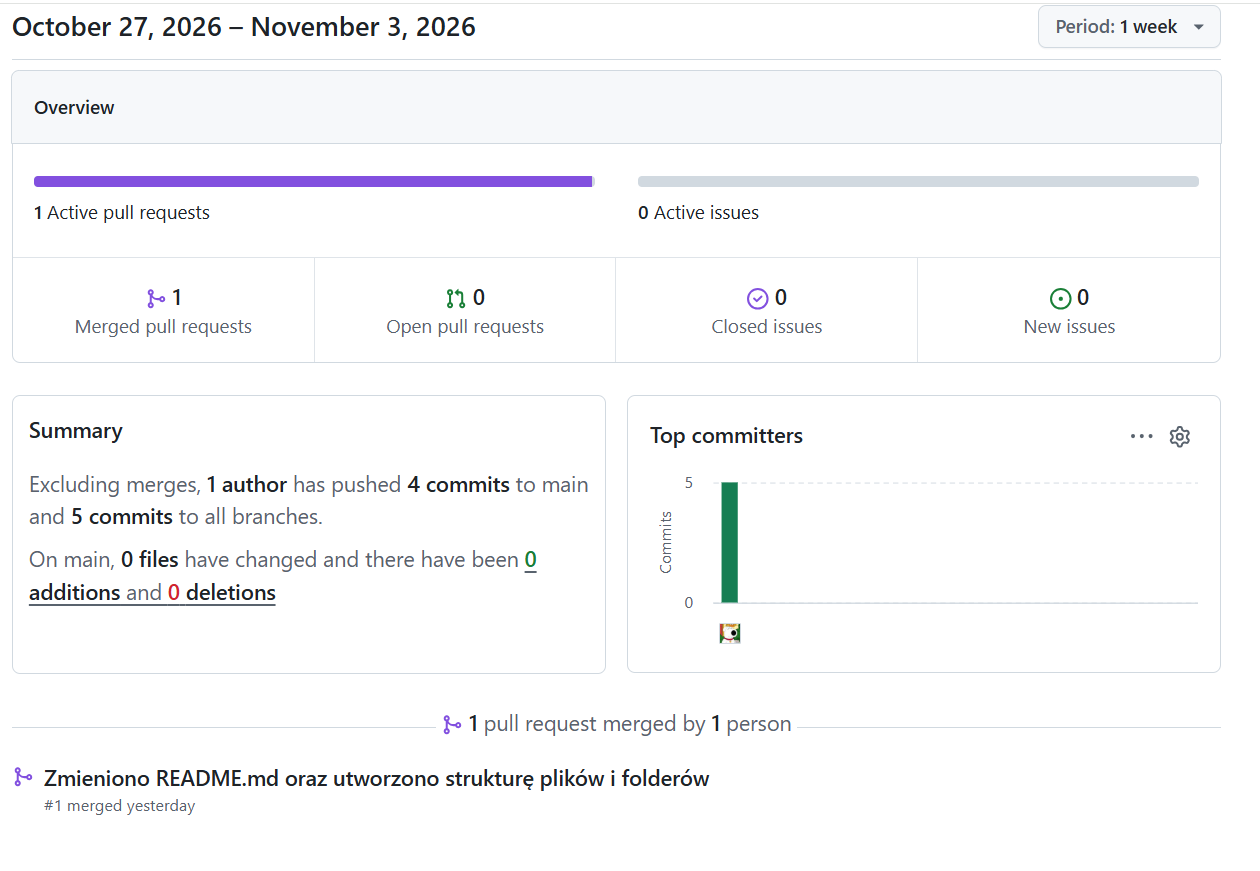
\includegraphics[width=0.75\linewidth]{rys/img1.png}
		\caption{Wizualizacja historii commitów i scalania gałęzi z platformy GitHub}
		\label{rys:rysunek001}
	\end{center}
\end{figure}

\subsection{Dokumentacja kodu za pomocą systemu Doxygen}

\hspace{0.60cm}
Do projektu należy dołączyć automatycznie wygenerowaną dokumentację techniczną. Wykorzystywany jest do tego system \textbf{Doxygen}, który agreguje specjalne bloki komentarzy umieszczone w plikach nagłówkowych \texttt{.h} i źródłowych \texttt{.cpp}.

\hspace{0.60cm}
Wykaz stosowanych tagów Doxygen przedstawia tabela \ref{tab:doxygen_tags} (s. \pageref{tab:doxygen_tags}).

\begin{tabela}
	{Najważniejsze znaczniki systemu Doxygen stosowane w dokumencie}
	{Najważniejsze znaczniki systemu Doxygen stosowane w dokumencie}
	{
		\begin{tabular}{|l|p{9.5cm}|} \hline
			\textbf{Znacznik Doxygen} & \textbf{Opis i funkcja w dokumencie} \\ \hline
			\texttt{@file} & Oznacza plik źródłowy lub nagłówkowy podlegający indeksowaniu. \\ \hline
			\texttt{@class} & Opisuje przeznaczenie i zakres odpowiedzialności danej klasy. \\ \hline
			\texttt{@brief} & Krótki, jednozdaniowy opis metody lub struktury. \\ \hline
			\texttt{@param} & Opisuje parametr wejściowy przekazywany do metody. \\ \hline
			\texttt{@return} & Opisuje wartość zwracaną przez funkcję lub metodę. \\ \hline
		\end{tabular}
	}
	\label{tab:doxygen_tags}
\end{tabela}

\hspace{0.60cm}
Podsumowując, zrealizowany w powyższy sposób rozdział wprowadza w kompletny zakres wymagań projektowych. Wszystkie operacje na drzewie BST, obsługa plików binarnych oraz procedury gitowe zostaną w kolejnych rozdziałach poddane szczegółowej analizie implementacyjnej i testowej.